\section{ SR01NL22 }


\subsection{Meta}

    \textbf{Title:}
    AI for patient scheduling in the real-world health care setting: A metanarrative review

    \begin{table}[H]
        \centering
        \begin{tabular}{|c|c|c|c|c|c|c|c|c|}
            \hline
                \textbf{Rank} & \textbf{Grasp} & \textbf{Grade} & \textbf{Type} & \textbf{Outcome} & \textbf{Domain} & \textbf{COV19} & \textbf{CoI} & \textbf{DB} \\
            \hline
                4 & 95\% & B & A & P & A & Yes & ?? & No \\
            \hline
        \end{tabular}
        \caption{Reference's metadata}
        \label{tab:SR01NL22}
    \end{table}

\subsection{Summary}
This article presents a systematic literature review that covers the natural language process models for predicting healthcare-related events from textual data. Oscar Hoekstra, William Hurst, and Joep Tummers conducted a quantitative analysis of the existing literature in the field by 2022. The authors emphasise that they are not comparing the existing studies due to the unavailability of the unified criteria but explore the performance of the NLP models separately. The work is well structured, but what needs to be added is a discussion on the healthcare problems which can be solved or optimised by the NLPs. 
    

\subsection{Notes}
    \begin{itemize}
        \item PubMed, IEEE and WebOfScience;
        \item Quality assessment method?
    \end{itemize}


\subsection{Reading}
    \textbf{Abstract:}
    The systematic literature review is summarising the results and show currnt efficiency of the Natural Language Processing models in the area of healthcare related event prediction. The authors used open access databases to retreave the corresponding studies. The current state of the research does not allow to make a comprehencive comparison of the existing solutions.
    
    \textbf{Objectives:}
    This research aims to investigate a medical event prediction solution with textual data on the input.

    \textbf{Page 1:}
    There are a lot of textual medical records which requre a lot of time and resources to structure in order to get some usefull insights. The current research looks into the NLP prediction models which use these type of records to predict healthcare related events.    
    
    \textbf{Page 2:}
    In the begining of the page, the authors formulate three questions for the research: What is the state-of-the-art? How do ML models predict? What ML models are sued? Then the outline of the paper is presented. The rest of the page describes the methodology methods used to search and screen the studies related to the topic.

    \textbf{Page 3:}
    The stages of the literature analysis are outlined and after the applying the selection methods the 38 articles have been selecet.
    \begin{figure}[H]
        \centering
        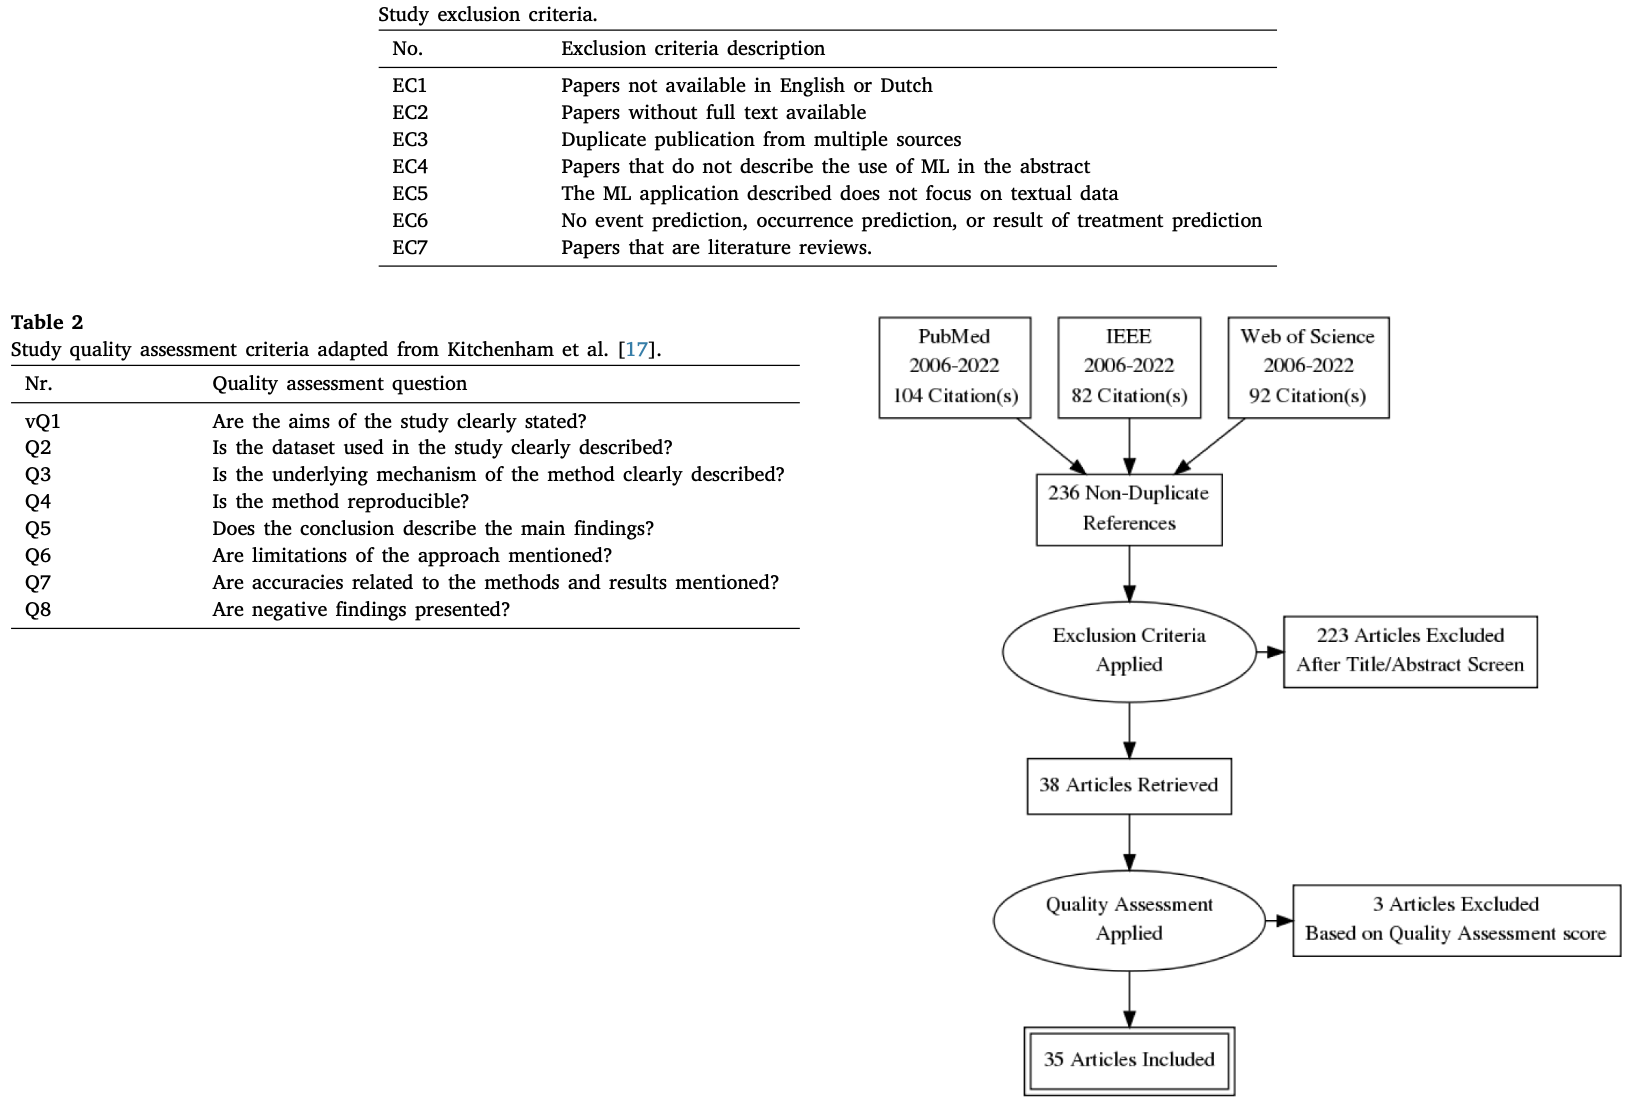
\includegraphics[width=1\textwidth]{figures/0009_SR01NL22/fig1.png}
        \caption{Selection critaria in \cite{x349}.}
        \label{fig1:0009_SR01ES23}
    \end{figure}

    \textbf{Page 4:}
    The quality evaluation results show that only one of nine papers is qualified. Also the performance critaria were presentd for the researched NLP models. 
    \begin{figure}[H]
        \centering
        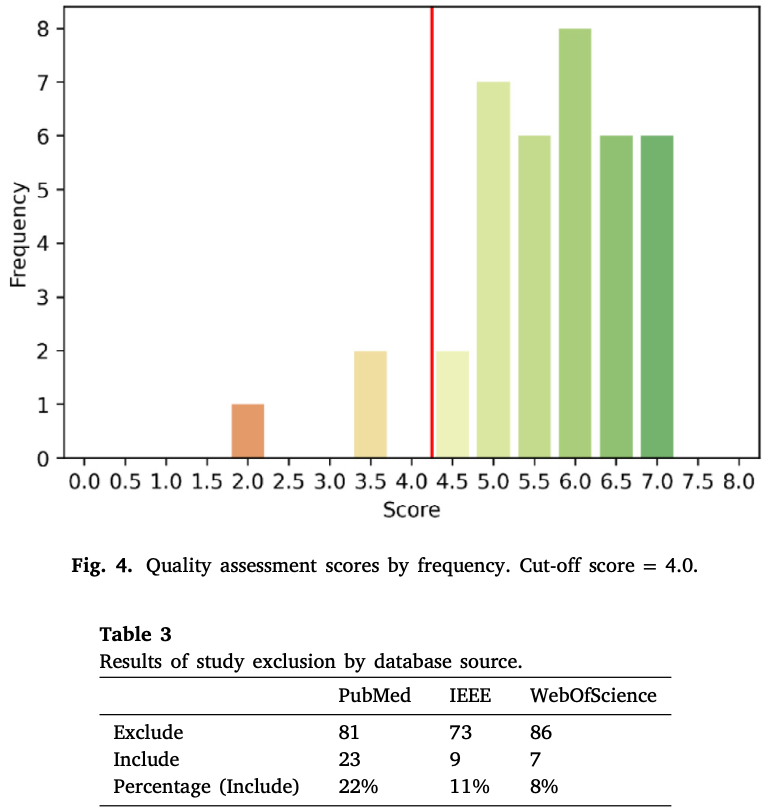
\includegraphics[width=.51\textwidth]{figures/0009_SR01NL22/fig2.png}
        \caption{Quality evaluation in \cite{x349}.}
        \label{fig2:0009_SR01ES23}
    \end{figure}
    \begin{figure}[H]
        \centering
        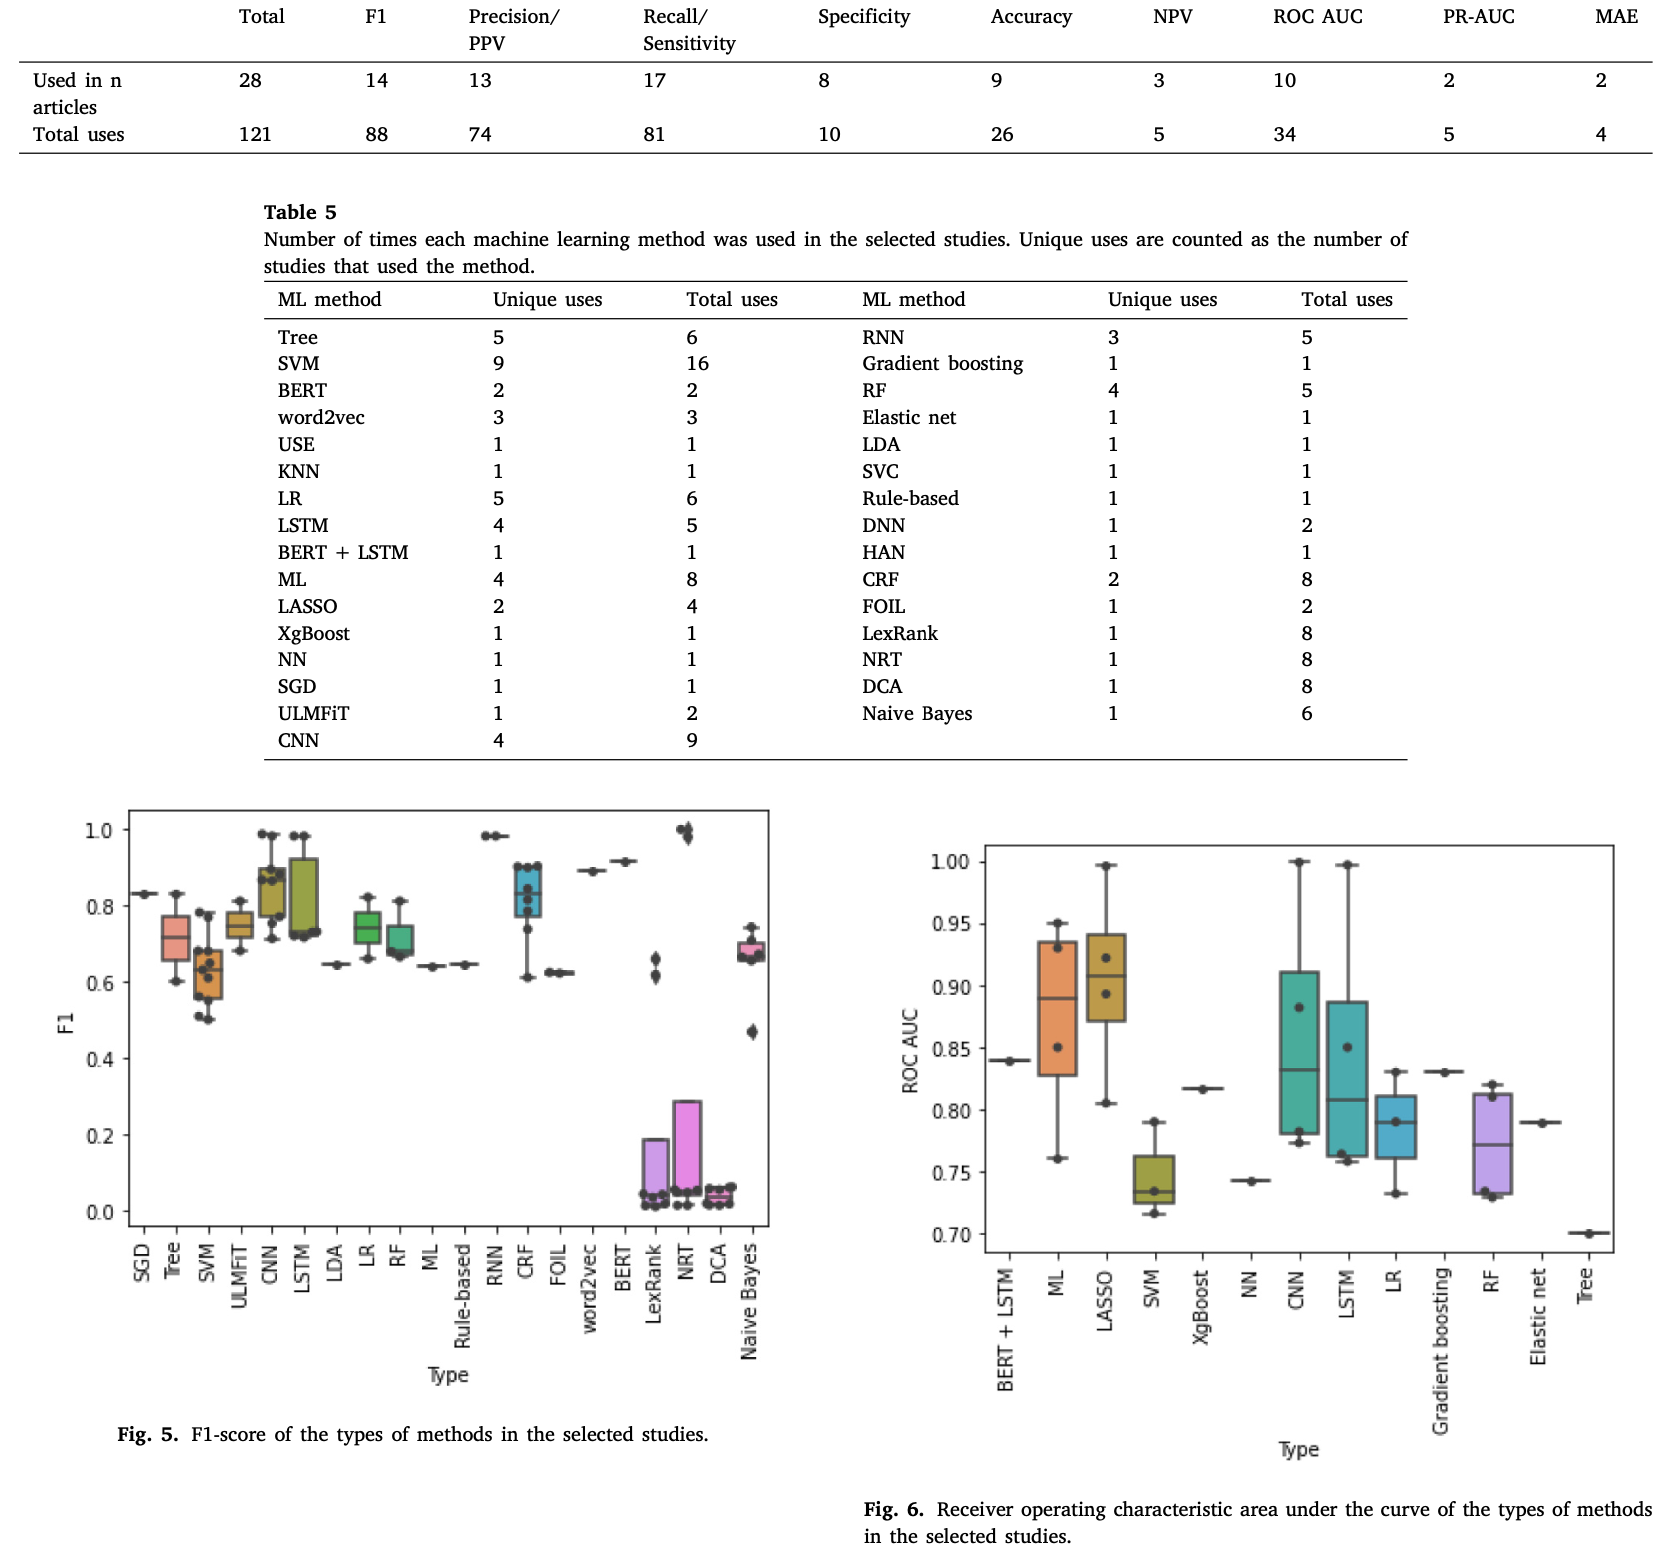
\includegraphics[width=1\textwidth]{figures/0009_SR01NL22/fig3.png}
        \caption{Method used distribution from \cite{x349}.}
        \label{fig3:0009_SR01ES23}
    \end{figure}

    \textbf{Page 5:}
    The SLR is the first in a kind according to the authors of the work. An interest in NLP technology is growing which is shown by the high publication rate for the last 5 years in comparison to earlier publications.
    
    \textbf{Page 5:}
    There is no ultimate supaeiar MLP model which will outperform the other solutions. There NLPs which can perform using just textual data, but for most cases the additional structured data is used to enhance the results. Till the end of the page the authors summarise the scores of different models and overal quality of the studies by the number of selected publications.
    \begin{figure}[H]
        \centering
        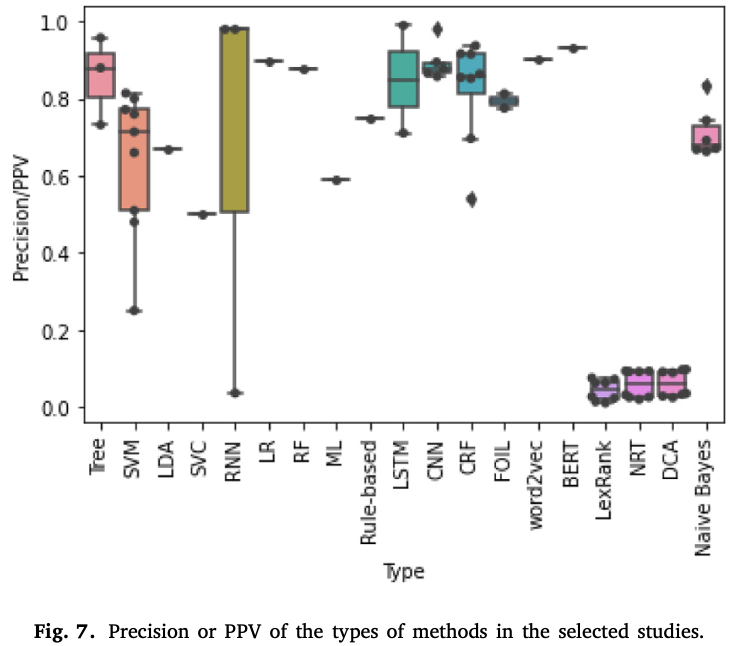
\includegraphics[width=.55\textwidth]{figures/0009_SR01NL22/fig4.png}
        \caption{Precision or PPV of the types of methods in the selected studies from \cite{x349}.}
        \label{fig4:0009_SR01ES23}
    \end{figure}
    \begin{figure}[H]
        \centering
        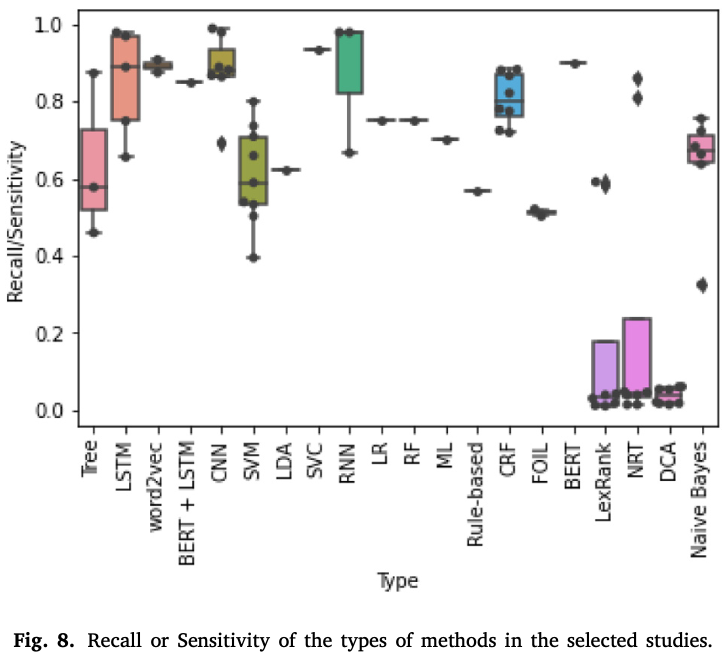
\includegraphics[width=.55\textwidth]{figures/0009_SR01NL22/fig5.png}
        \caption{Recall or Sensitivity of the types of methods in the selected studies from \cite{x349}.}
        \label{fig5:0009_SR01ES23}
    \end{figure}
    
    \textbf{Page 6:}
    There are multiple obsticles to the conducting this systematic literature review. First some studies present unexpected unrealistic results lik F1-score above. Another challenge were studies which do not evaluate their models. 
    \begin{figure}[H]
        \centering
        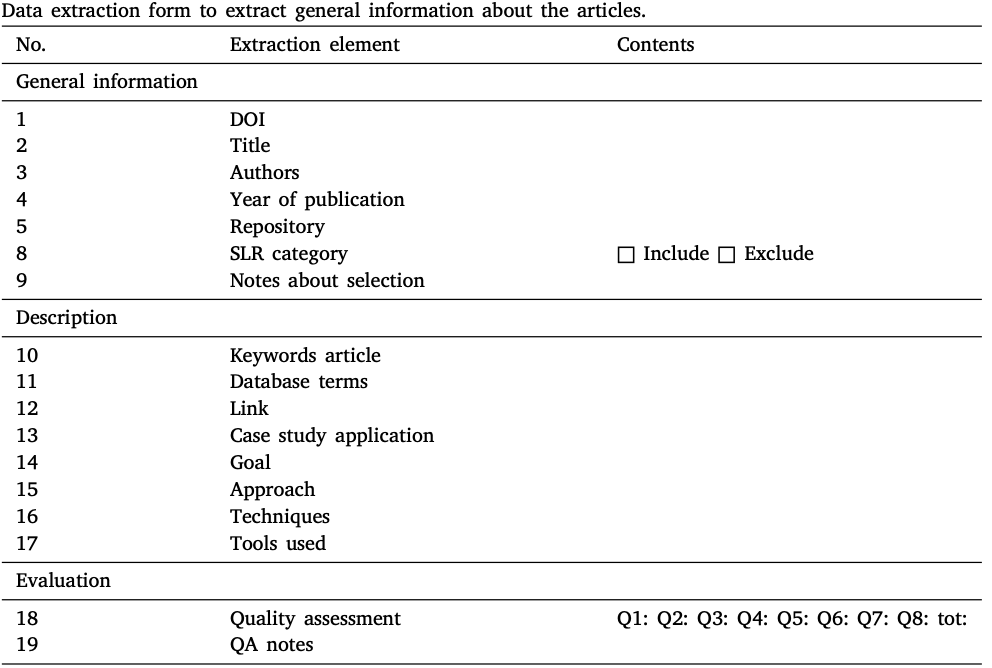
\includegraphics[width=1\textwidth]{figures/0009_SR01NL22/fig6.png}
        \caption{Extructed data from publication in \cite{x349}.}
        \label{fig6:0009_SR01ES23}
    \end{figure}
    
    \textbf{Conclusion:}
    In the conclusion the authors hihglighted stable good performance of the Neural Network models and also BERT models. The all outilined in the introduction aims were reached and the suggestion for the future research is to standardise the evaluation criteria for the NLP models.
